\documentclass{standalone}
\usepackage{protocol}
\usepackage{amsfonts}
\usepackage{amsmath}
\usepackage{graphicx}	
\usepackage{tikz}	

%---------------IKE abbreviations-----------------
\newcommand{\ckyi}{\ensuremath{\mathsf{SPI_I}}}
\newcommand{\ckyr}{\ensuremath{\mathsf{SPI_R}}}

%-------------cryptographic primitives-----------------
\newcommand{\PRF}[2]{\mathsf{PRF}_{#1}(#2)}
\newcommand{\iprf}[2]{\mathsf{IPRF}_{#1}(#2)}
\newcommand{\MAC}[2]{\mathsf{MAC}_{#1}(#2)}
\newcommand{\SE}{\mathsf{SE}}
\newcommand{\Enc}{\mathsf{Enc}}
\newcommand{\Dec}{\mathsf{Dec}}
\newcommand{\ENC}[2]{\mathsf{Enc}_{#1}(#2)}
\newcommand{\DEC}[2]{\mathsf{Dec}_{#1}(#2)}
\newcommand{\Decrypt}{\mathsf{Decrypt}}
\newcommand{\Encrypt}{\mathsf{Encrypt}}
\newcommand{\SIGN}{\mathsf{Sign}}
\newcommand{\Vfy}{\mathsf{Vfy}}
\newcommand{\Hash}{\mathsf{h}}
\newcommand{\PKE}{\mathsf{PK.Enc}}
\newcommand{\PKD}{\mathsf{PK.Dec}}


%---------------Algo-------------------
\newcommand{\rand}{\stackrel{{\scriptscriptstyle\$}}{\leftarrow}}
\newcommand{\bits}{\{0,1\}}

\begin{document}




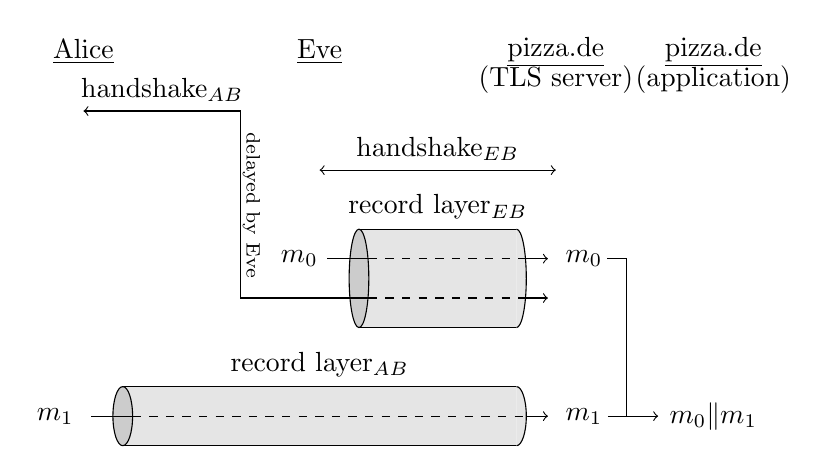
\begin{tikzpicture}
\draw (0,0.25) node {\underline{Alice}};
\draw (3,0.25) node {\underline{Eve}};
\draw (6,0.25) node {\underline{pizza.de}};
\draw (6,-0.1) node {(TLS server)};
\draw (8,0.25) node {\underline{pizza.de}};
\draw (8,-0.1) node {(application)};
% handshake_{EB}
\draw[<->] (3,-1.25)--(6,-1.25);
\draw (4.5,-1.25) node[above] {handshake$_{EB}$};
% record layer_{EB} cylinder
\draw (4.5,-2) node[above] {record layer$_{EB}$};
\fill[gray!20!white] (3.5,-2)--(5.5,-2)--(5.5,-3.25)--(3.5,-3.25)--(3.5,-2);
\draw (3.5,-2)--(5.5,-2);
\draw (3.5,-3.25)--(5.5,-3.25);
\fill[gray!40!white] (3.5,-2.625) circle[x radius=0.125, y radius=0.625];
\draw (3.5,-2.625) circle[x radius=0.125, y radius=0.625];
\fill[gray!20!white] (5.5,-2) arc[start angle=90,end angle=-90,x radius=0.125, y radius=0.625];
\draw (5.5,-2) arc[start angle=90,end angle=-90,x radius=0.125, y radius=0.625];
% m_{0}
\draw (3.1,-2.375)--(3.625,-2.375);
\draw[dashed] (3.625,-2.375)--(5.625,-2.375);
\draw[->] (5.625,-2.375)--(5.9,-2.375);
\draw (3.1,-2.375) node[left] {$m_{0}$};
\draw (6.0,-2.375) node[right] {$m_{0}$};
% handshake_{AB}
\draw[<-] (0,-0.5)--(2,-0.5)--(2,-2.875)--(3.625,-2.875);
\draw[dashed] (3.625,-2.875)--(5.625,-2.875);
\draw[->] (5.625,-2.875)--(5.9,-2.875);
\draw (1,-0.5) node[above] {handshake$_{AB}$};
\draw (1.9,-1.7) node[right] {\rotatebox{270}{\scriptsize delayed by Eve}};
% record layer_{AB} cylinder
\draw (3,-4) node[above] {record layer$_{AB}$};
\fill[gray!20!white] (0.5,-4)--(5.5,-4)--(5.5,-4.75)--(0.5,-4.75)--(0.5,-4);
\draw (0.5,-4)--(5.5,-4);
\draw (0.5,-4.75)--(5.5,-4.75);
\fill[gray!40!white] (0.5,-4.375) circle[x radius=0.125, y radius=0.375];
\draw (0.5,-4.375) circle[x radius=0.125, y radius=0.375];
\fill[gray!20!white] (5.5,-4) arc[start angle=90,end angle=-90,x radius=0.125, y radius=0.375];
\draw (5.5,-4) arc[start angle=90,end angle=-90,x radius=0.125, y radius=0.375];
% m_{1}
\draw (0.1,-4.375)--(0.625,-4.375);
\draw[dashed] (0.625,-4.375)--(5.625,-4.375);
\draw[->] (5.625,-4.375)--(5.9,-4.375);
\draw (0,-4.375) node[left] {$m_{1}$};
\draw (6,-4.375) node[right] {$m_{1}$};
% m_{0} || m_{1}
\draw (6.65,-2.375)--(6.9,-2.375)--(6.9,-4.375);
\draw[->] (6.66,-4.375)--(7.3,-4.375);
\draw (8,-4.375) node {$m_{0} \| m_{1}$};
\end{tikzpicture}




\end{document}